\documentclass[12pt,t]{beamer}
\usetheme[nat,
  % Ændre til NAT, KU, eller unit=ics (diku)
  dk, % Sprog
  %style=simple, % Vandmærke eller billede
  footstyle=low, % Fjern stor footer
  wmark, % vandmærke på hver side
  logoplace=left % Logo til venstre
  %,sidebar % makes sidebar
]{Frederiksberg}
% nat for Science, ku for generic or unit=ics for DIKU
% Tilføj style=simple for vandmærke
\usepackage{listings} % Pakke til kode
\usepackage{pslatex}        % pæn skrift
\usepackage[utf8]{inputenc} % Implementerer Unicode
\usepackage{algpseudocode}
\usepackage{algorithm}

\title{Studiepraktik 2018}
\subtitle{Øvelser i Algoritmer og problemløsning}
\author{
  Benjamin Rotendahl  \\
}

\date[]{\today}


\begin{document}

\frame[plain]{\titlepage}
\frame{\tableofcontents}


\begin{frame}
  \frametitle{Program for idag}
  \begin{block}{Fra nu til 11.50}
    \begin{itemize}
      \item Øvelser i algoritmer \pause
      \item Sjove gåder \pause
      \item Opsamling og spørgsmål
    \end{itemize}
  \end{block}
\end{frame}


\section{Algoritme vs Algoritme}
\begin{frame}[t]{Valget af algoritme}
  \begin{exampleblock}{Soterings algoritmer}
    Givet en liste af $n$ tal ønsker vi at returnere en sorteret liste
    af længde $n$.
  \end{exampleblock}
  \pause
  \vspace{-2em}
  \begin{columns}
    \begin{column}{0.5\textwidth}
      \begin{block}{Hold $A$}
        \begin{itemize}
          \onslide<+->{\item Har en computer}
                \onslide<+->{\item Bruger algoritmen \emph{Merge Sort}}
                \onslide<+->{\item De kan sortere $10$ millioner tal på
                under $20$ minutter}
                \onslide<+->{\item De kan sortere $100$ millioner tal på
                $4$ timer.}
        \end{itemize}
      \end{block}
    \end{column}
    \begin{column}{0.5\textwidth}
      \begin{block}{Hold $B$}
        \begin{itemize}[<+->]
          \item Har en computer der er $1000$ gange hurtigere end
                hold A
          \item Bruger algoritmen \emph{Insertion Sort}
          \item De kan sortere $10$ millioner tal på $5$ timer.
          \item De kan sortere $100$ millioner tal på \alert{23 dage!}
        \end{itemize}
      \end{block}
    \end{column}
  \end{columns}
\end{frame}

\begin{frame}[t]{Eksempler på køretid}
  \vspace{-2em}
  \begin{columns}
    \begin{column}{0.33\textwidth}
      \begin{block}{Bogo Sort}
        \begin{itemize}
          \item Køretid på $O(n!)$
        \end{itemize}
      \end{block}
    \end{column}
    \begin{column}{0.33\textwidth}
      \begin{block}{Insertion Sort}
        \begin{itemize}
          \item Køretid? $O(n^2)$
        \end{itemize}
      \end{block}
    \end{column}

    \begin{column}{0.33\textwidth}
      \begin{block}{Merge sort}
        \begin{itemize}
          \item Køretid på $O(n \lg n)$
        \end{itemize}
      \end{block}
    \end{column}
  \end{columns}
  \begin{figure}[h!]
    \caption{Graf over køretider}
    \centering
    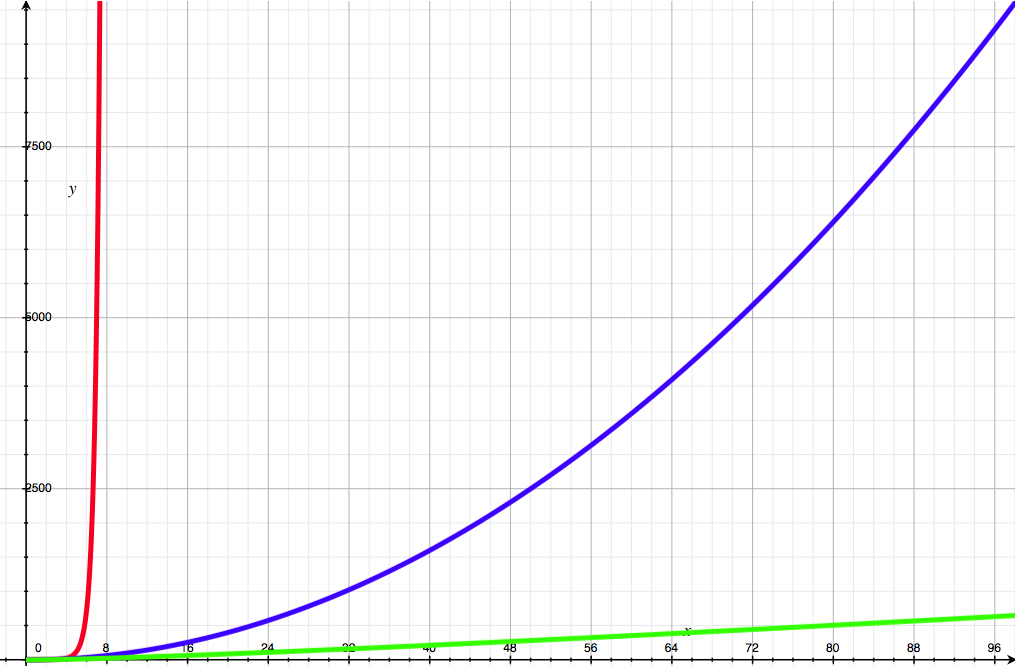
\includegraphics[width=0.7\textwidth]{./include/exs.png}
  \end{figure}
\end{frame}

\begin{frame}[t]{Sammenligning af Algoritmer}
  \begin{quote}
    Vi bruger begrebet \emph{Køretid} for at beskrive hvordan tiden en
    algoritme bruger stiger med input.
  \end{quote}
  \pause
  \vspace{-1em}
  \begin{block}{Definition på køretid}
    En øvregrænse for den tid der bliver brugt på at løse et problem af
    størelse $n$. Skrives som
    $$
      O(n), O(n^2), O(n \lg n), O(n!), O\left( \frac{a}{b} \right)
    $$
  \end{block}
  \pause
  \begin{exampleblock}{Algoritme for minimums funktionen}
    Givet en liste $X = [x_1,x_2,\dots,x_n]$ ønsker vi at returnere det
    mindste tal i listen. Hvad er algoritmen og hvad er køretiden?
  \end{exampleblock}
\end{frame}

\begin{frame}{Minimums algoritme}
  \begin{block}{Eksempel}
    \vspace{-1.5em}
    \begin{algorithm}[H]
      \caption{\newline Input: En liste $X=[x_1,x_2, \dots, x_n]$
      \newline Ouput: Det mindste tal i listen.
      }
      \begin{algorithmic}
        \State min = $x_1$
        \For{$x_i$ in X}
        \If{$x_i < \min$}
        \State min = $x_i$
        \EndIf
        \EndFor
      \end{algorithmic}
    \end{algorithm}
  \end{block}
  \pause
  \begin{block}{Analyse af algoritmen}
    \centering Køretid? \pause $O(n)$ \\
    \pause
    \centering Er den optimal? \pause \alert{Jeps!}
  \end{block}
\end{frame}


\section{Algoritme design}
\begin{frame}[c]{Hvordan finder man på en algoritme}
  \begin{block}{Algoritme for algoritmer}
    \begin{enumerate}
      \item Beskriv problemet med egne ord. \pause
      \item Del problemet op i mindre dele. \pause
      \item Definer input \pause
      \item Definer output \pause
      \item Beskriv trin for at gå fra input til output
    \end{enumerate}
  \end{block}
\end{frame}

\section{Øvelser}
\begin{frame}[t]{Øvelser}
  \begin{block}{Algoritme for øvelserne}
    \begin{enumerate}
      \item Der præsenteres et problem med eksempler. \pause
      \item I finder på en algoritme for problemet
            (Arbejd gerne sammen) \pause
      \item Vi løser den sammen på tavlen. \pause
      \item Plus gåder!
    \end{enumerate}
  \end{block}
\end{frame}

\begin{frame}
  \frametitle{Søgning}
  \begin{block}{Mål}
    Givet en sorteret liste og et element, bestem om element er i listen,
    ved at kigge på så få elementer som muligt.
  \end{block}
  \pause

  \begin{exampleblock}{Eksempel}
    Lad en liste være givet ved $[2, 4, 5, 7, 8, 11, 25]$, hvor vi ønsker at
    finde ud af om elementet 11 er listen. Svaret skulle gerne være ja.
    (det første element har indeks 0).
  \end{exampleblock}
\end{frame}

\begin{frame}
  \frametitle{Sortering}
  \begin{block}{Mål}
    Sorter en givet usorteret liste.
  \end{block}
  \pause

  \begin{exampleblock}{Eksempel}
    Lad en liste være givet ved [7, 4, 5, 12, 1], denne vil vi gerne sortere!
    Den sorterede liste skulle gerne være [1, 4, 5, 7, 12].
  \end{exampleblock}
\end{frame}


\begin{frame}{Nøgle gåde}
  \begin{block}{Hvordan holder jeg min garagedør lukket?}
    I har en gargeport med en IR modtager der kan modtage et
    signal og en nøglering der kan sende et signal.
  \end{block}\pause
  \begin{block}{Mål}
    Hvordan kan vi gøre den sikker? Hvad skal ``Computeren'' i
    nøgleringen kunne?
  \end{block}
  \pause
  \begin{exampleblock}{Eksempel}
    Send en kode til IR modtageren?
  \end{exampleblock}
\end{frame}


\begin{frame}[c]{Overlappende under problemer}
  \begin{block}{Eksempel}
    Det $n$'te\emph{Fibonacci} tal er defineret som summen af de to
    forgående.
    $$
      1,1,2,3,5,8,13,21,34,55, \dots
    $$
    \pause
    Hvordan bestemmer vi dem?
  \end{block}
\end{frame}

\begin{frame}[c]{Sommer i Sunny beach}
  \begin{block}{Beskrivelse}
    Det er sommer i \emph{Sunny Beach} og en kæde af barer langs kysten
    har et problem,\pause  de kan ikke bestille flere øl!
    \\
    \pause  ~ \\
    Hver bar langs strandvejen har $b_i$ øl tilbage, der er ikke
    nogen der ved hvilken bar der kan sælge flest øl på en given aften.
    \pause
    Det er besluttet at alle barer skal have lige mange øl. \\
    \pause
    ~\\
    De har en lastbil hvor der kan være en uendelig mængde af øl, \pause
    dog er vognførererne på denne lastbil glade for øl. Hver gang der er
    kørt en kilometer så drikkes der to øl.
  \end{block}
\end{frame}

\begin{frame}[c]{Eksempel}
  \begin{block}{Figur}
    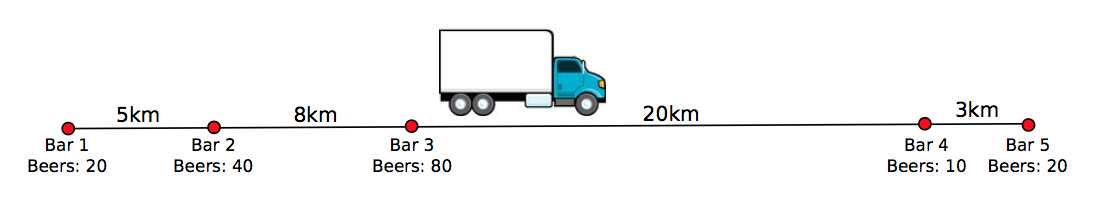
\includegraphics[scale=0.5]{include/fragt.png}
  \end{block}
  \pause
  \begin{block}{Hvad i får som input}
    \begin{itemize}
      \item En liste over hvor mange øl der er på hver bar $b_1, b_2, \dots$
      \item En liste over afstanden mellem dem $a_1, a_2, \dots$ \pause
      \item Det antal øl de gerne vil have på hver bar \pause
    \end{itemize}
  \end{block}

  \begin{block}{Hvad i skal svare}
    \begin{itemize}
      \item ja, eller nej. \pause
      \item Svar også på hvordan man kan finde det optimale antal.
    \end{itemize}
  \end{block}
\end{frame}

\begin{frame}{DNS system}
  \begin{block}{Hvad er DNS}
    Forklaring på tavlen
  \end{block}
  \begin{block}{Mål}
    Tænk over hvordan vi kan lave et DNS system
  \end{block}
  \pause
  \begin{exampleblock}{Eksempel}
    Snak lidt om hvordan det kunne gøre smart
  \end{exampleblock}
\end{frame}

\begin{frame}[plain]{Zig-Zag sekvens}
  \begin{block}{Beskrivelse}
    Ejeren af et supermarked har fået en ny stor ølhylde, nu vil han gerne
    gøre den pæn. Han har placeret sine øl i alfabetisk orden, men højden
    på flaskerne afviger. Han er nu intereseret i at finde den længste
    sekvens af øl der skifter mellem lav og høj en såkaldt Zig-Zag sekvens.
    Så $(15,10,17)$ er sådan en sekvens mens $(1,2,3)$ ikke er.

    Vi skal lave en algoritme der bestemmer sådan en sekvens.\\
    \textbf{Input:} $n$ øl flaskers højde $n_1, n_2, \dots$. \\
    \textbf{Output:} Den længst mulige Zig-Zag sekvens.
  \end{block}
\end{frame}

\begin{frame}
  \begin{columns}
    \begin{column}{0.5\textwidth}
      \begin{block}{Eksempel}
        \begin{itemize}
          \item Input : $(6, 1, 7, 7, 2, 4, 7)$
          \item Output : $(6,1,7,2,7)$
        \end{itemize}
      \end{block}
    \end{column}
    \begin{column}{0.5\textwidth}
      \begin{block}{Figur}
        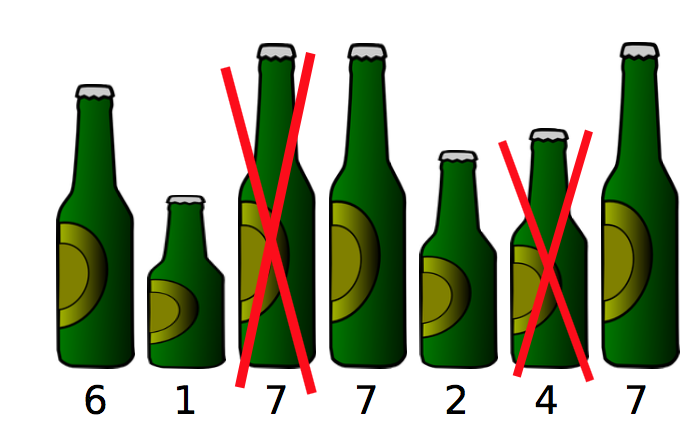
\includegraphics[scale=0.3]{include/oel.png}
      \end{block}
    \end{column}
  \end{columns}
  I må gerne fjerne flasker men ikke bytte rundt på dem, beskriv en metode
  til at bestemme den her sekvens og tænk over hvor effektivt den er.
\end{frame}


\begin{frame}{Primtal}
  \begin{block}{Mål}
    Skriv en algoritme der finder det $n$'te primtal --- prøv at gør den så
    hurtig som mulig.
  \end{block}
  \pause

  \begin{exampleblock}{Eksempel}
    Find det femte primtal. Algoritmen skal gerne returnere 11.
  \end{exampleblock}
\end{frame}


\end{document}
